\section{Task 1 - Basic layout}

\begin{frame}{Task 1 - Basic Layout}
    If you haven't, get the source code from the \href{https://github.com/NEEECFEUP/WS-App-Development/}{Github Repository}.

    \begin{block}{Hint!}
        To print to the terminal, use:
        
        \mint{dart}| import 'dart:developer' as developer;|

        and

        \mint{dart}| developer.log('Hello!', name: 'app.log');|
    \end{block}
\end{frame}

\begin{frame}{Task 1 - Basic Layout}
    \begin{itemize}
        \item Create a screen with a Text "Hello World"
        \item A button "Click" under it
        \item When you click the button, print something to the terminal
    \end{itemize}
\end{frame}

\begin{frame}{Task 1 - Basic Layout}
    \begin{figure}[h]
        {
            \setlength{\fboxsep}{0pt}%
            \setlength{\fboxrule}{0.5pt}%
            \fbox{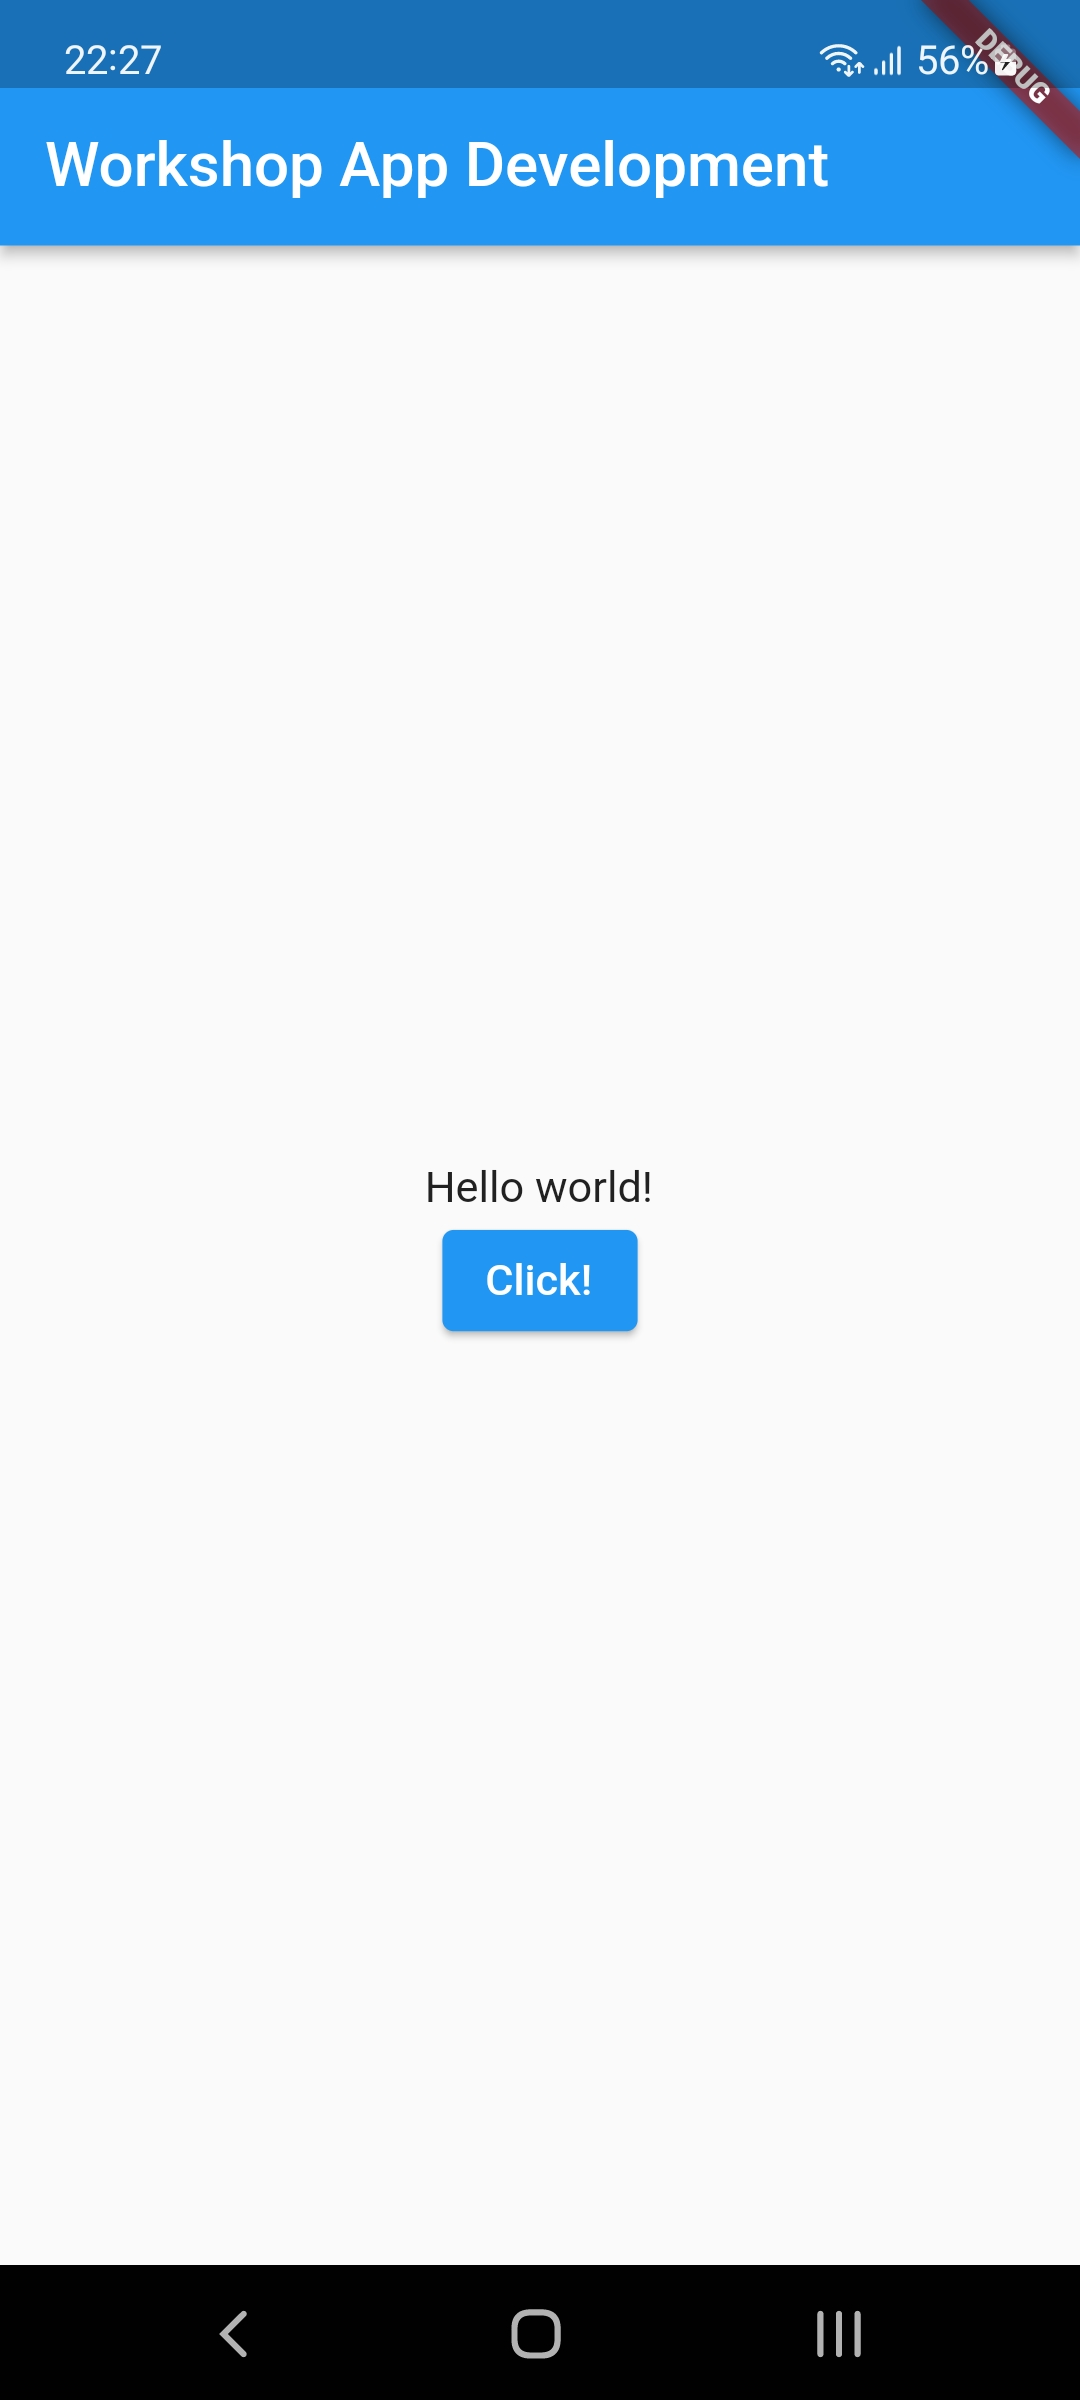
\includegraphics[width=0.3\textwidth]{images/task1.jpg}}
        }
    \end{figure}
\end{frame}

\begin{frame}{Task 1 - Basic Layout}
    \begin{figure}[h]
        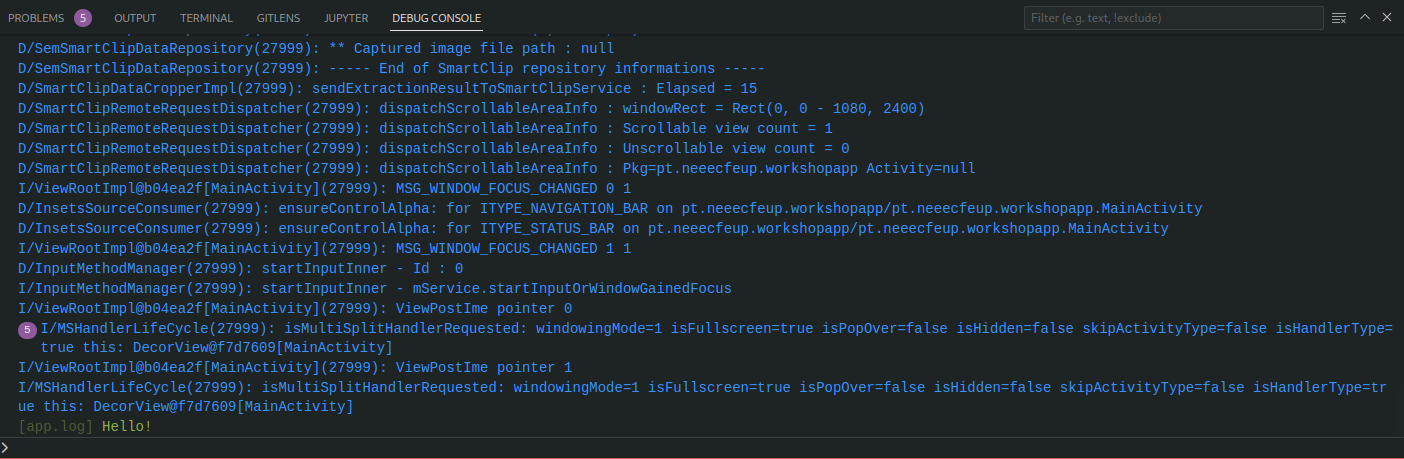
\includegraphics[width=1\textwidth]{images/task1-term.png}
    \end{figure}
\end{frame}